
\subsection{Modifications on prediction}

\paragraph{Models}

\delete{Use Auto-regression \& seasonality}
\begin{align}
x(y, day+d\_ah,hr) = \sum_{a=0}^{A-1} \omega_a x(y, day-a,hr) \nonumber \\
+ \sum_{mo=1}^{M} \upsilon_{mo} \bar{x}(y-1, mo, hr) + c
\end{align}

\delete{Implementation problems: (1) cannot find the right tool for it, (2) we do not have enough data to do it (only 3 year data).}

We use SVM with the following features for
\begin{itemize}
	\item solar \& wind: latest 7 days before 30 day ahead, month of year, day of month, and hour of day.	
	\item prices: month of year, day of month, day of week, and hour of day. (do not use latest 7 days before 30 day ahead which even cause much larger errors).
	\item workload: latest 7 days before 2 day ahead, day of week, and hour of day.
\end{itemize}

\paragraph{Argument for large errors of long-term forecast}
\begin{itemize}
	\item Long-term feature data are not available. Long-term forecast for weather is very complex which requires the data from many parts of the world which is only available in some specialized centers \cite{wmoLongTermForecasting}.
	\item Simple methods do not succeed. The simpler ways based on the work out rules, using statistics, linking the future patterns to the current features do not work well. 
	\item Low correlation between the past data and the future data. For example, the prices in Ohio significantly change in year 2009 due to the new policy.
\end{itemize}

cite some works on renewable energy, and electricity prices in long-term: electricity prices \cite{hyndman2010density} , energy demand \cite{nowotarski2013robust}

\begin{figure}[!t]
	\centering
	\subfloat[PV generation]{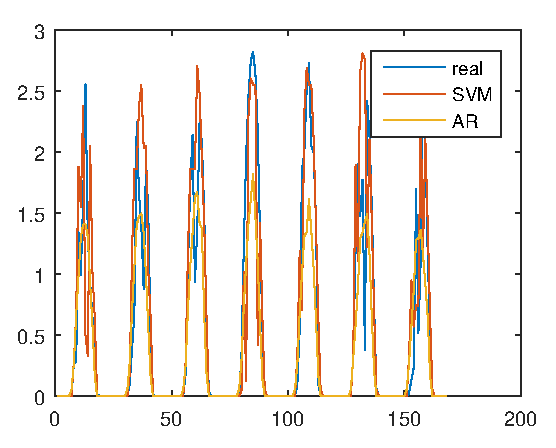
\includegraphics[width=.5\linewidth]{figs/predicted_solar}}
	\subfloat[Wind generation]{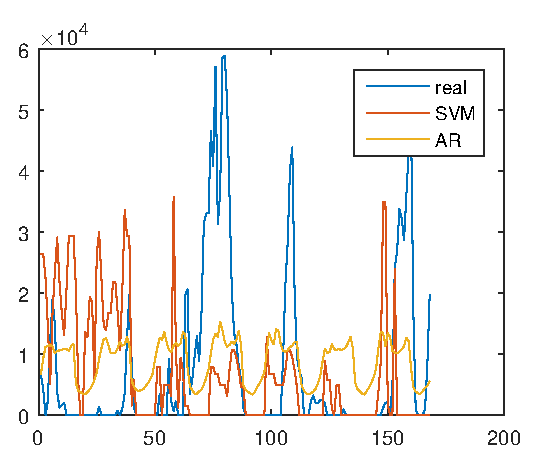
\includegraphics[width=.5\linewidth]{figs/predicted_wind}}
	\\
	\subfloat[Electricity price]{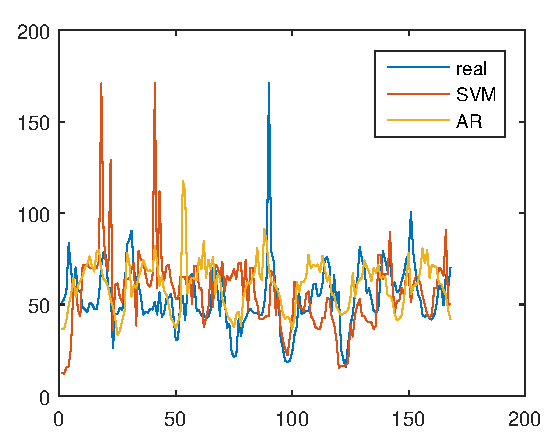
\includegraphics[width=.5\linewidth]{figs/predicted_prices}}
	\subfloat[Workload]{
\includegraphics[width=.5\linewidth]{figs/blank}}
	\caption{Predicted vs. actual.}
	\label{fig:PredictVsActual}
\end{figure}

\begin{figure}[!t]
	\centering
	\subfloat[PV generation]{\includegraphics[width=.5\linewidth]{figs/svm_vs_ar_vs_avg_solar}}
	\subfloat[Wind generation]{\includegraphics[width=.5\linewidth]{figs/svm_vs_ar_vs_avg_wind}}
	\\
	\subfloat[Electricity price]{\includegraphics[width=.5\linewidth]{figs/svm_vs_ar_vs_avg_price}}
	\subfloat[Workload]{\includegraphics[width=.5\linewidth]{figs/svm_vs_ar_vs_avg_workload}}
	\caption{RMSE comparisons.}
	\label{fig:CompareRMSE}
\end{figure}


\begin{figure}[!t]
	\centering
	\subfloat[PV generation]{\includegraphics[width=.5\linewidth]{figs2/svm_vs_ar_vs_avg_solar}}
	\subfloat[Wind generation]{\includegraphics[width=.5\linewidth]{figs2/svm_vs_ar_vs_avg_wind}}
	\\
	\subfloat[Electricity price]{\includegraphics[width=.5\linewidth]{figs2/svm_vs_ar_vs_avg_price}}
	\subfloat[Workload]{\includegraphics[width=.5\linewidth]{figs2/svm_vs_ar_vs_avg_workload}}
	\caption{MAE (mean absolute error) comparisons.}
	\label{fig:CompareMAE}
\end{figure}